%%%%%%%%%%%%%%%%%%%%%%
% This is an example presentation made with Christopher Gandrud's unofficial LSE Beamer theme
% Updated 27 December 2011
%%%%%%%%%%%%%%%%%%%%%%

\documentclass[xcolor={svgnames,usenames}]{beamer}
\usetheme{LSE}
\usepackage{color}
\usepackage{hyperref}
\hypersetup{colorlinks=true,linkcolor=black}
\usepackage{graphics}
\usepackage{pgf,tikz,pgfplots}
\usetikzlibrary{shapes,arrows,intersections,tikzmark,backgrounds}
\usetikzlibrary{matrix,fit,calc,trees,positioning,arrows,chains,shapes.geometric,shapes}
\usetikzlibrary{decorations.pathmorphing,patterns}
\usepackage{booktabs}
\usepackage{minted}
\usepackage{nicefrac}

% ----------------
% Disegni Tikz per differenze finite
% ----------------
\pgfdeclarelayer{edgelayer}
\pgfdeclarelayer{nodelayer}
\pgfsetlayers{edgelayer,nodelayer,main}

\tikzstyle{none}=[inner sep=0pt]

\usetikzlibrary{decorations.markings}
\usetikzlibrary{shapes.geometric}

\tikzstyle{rn}=[circle,fill=Red,draw=Black,line width=0.8 pt,inner sep=0p]
\tikzstyle{gn}=[circle,fill=Lime,draw=Black,line width=0.8 pt]
\tikzstyle{yn}=[circle,fill=Yellow,draw=Black,line width=0.8 pt]

\tikzstyle{simple}=[-,draw=Black,line width=2.000]
\tikzstyle{arrow}=[-,draw=Black,postaction={decorate},decoration={markings,mark=at position .5 with {\arrow{>}}},line width=2.000]
\tikzstyle{tick}=[-,draw=Black,postaction={decorate},decoration={markings,mark=at position .5 with {\draw (0,-0.1) -- (0,0.1);}},line width=2.000]

%%%%%%%%%%%%%%%%%%%%%%%%%%%%%%%% Title Slide %%%%%%%%%%%%%%%%%%%%%%%%%%
\title[Calcolo Parallelo]{Calcolo Parallelo : Lezione 3}
\author[F. Durastante]{
	\href{mailto:fabio.durastante@unipi.it}{Fabio Durastante}
}
\institute{Dipartimento di Matematica, Università di Pisa}
\date[Maggio 2021]{Master in Scienze e Tecnologie Spaziali, 2021}

\beamerdefaultoverlayspecification{}

\begin{document}

\begin{frame}
	\titlepage
\end{frame}

\section[Outline]{}
\frame{\tableofcontents}

%%%%%%%%%%%%%%%%%%%%%%%%%%%%%%%%%
\section{Some advanced instructions}

\subsection{Derived datatypes}
\begin{frame}{Derived datatypes}
	All the communication procedures we have seen until now are built on the assumption that
	\begin{itemize}
		\item all the buffers contain a sequence of identical \emph{basic} datatypes.
	\end{itemize}
	This is constraining, sometimes we need more flexibility, we may want to
	\begin{itemize}
		\item pass messages that contain values with different datatypes,
		\item send noncontiguous data
	\end{itemize}

\onslide<2->{We can define a \alert{general datatype} as an \emph{opaque} object specifying
	\begin{itemize}
		\item a sequence of basic datatypes,
		\item a sequence of integer (byte) displacements (that may not be positive, distinct or increasing in order)
	\end{itemize}
}
\begin{onlyenv}<3->
Such \textbf{sequence of pairs} is called then a \alert{type map}:
\begin{center}
Typemap = \{(\alert<4>{type$_0$} , \alert<5>{disp$_0$} ), \ldots , (\alert<4>{type$_{n-1}$} , \alert<5>{disp$_{n-1}$} )\},
\end{center}
where type$_i$ are \alert<4>{basic types}, and disp$_i$ are \alert<5>{displacements}.
\end{onlyenv}
\end{frame}

\begin{frame}{Derived datatypes}
Given a type map
\begin{center}
	Typemap = \{({type$_0$} , {disp$_0$} ), \ldots , ({type$_{n-1}$} , {disp$_{n-1}$} )\},
\end{center}
then
\begin{itemize}
	\item<1-> the \textbf{extent} of a datatype is defined to be the span from the first byte to the last byte
	occupied by entries in this datatype,\only<1>{ i.e., 
		\begin{flushleft}
			lb(Typemap) = $\min_j$disp$_j$,\\
			ub(Typemap) = $\max_j($disp$_j$ + sizeof$($tipe$_j)) + \varepsilon$,\\
			extent(Typemap) = ub(Typemap) - lb(Typemap),
		\end{flushleft}
	    in which the $\varepsilon$ is used to to satisfy alignment requirements.
	}
	\item<2-> The definition of extent is motivated by the assumption that the amount
	of \emph{padding added} at the end of each structure in an array of structures is \emph{the least
	needed} to fulfill alignment constraints.
	\item<3-> We need some \emph{constructor} routines to build and define the new datatypes.
\end{itemize}
\end{frame}

\begin{frame}[fragile]{Datatype constructors -- \mintinline{c}{MPI_TYPE_CONTIGUOUS}}
Allows for the replication of a datatype into contiguous locations.
\begin{minted}{c}
int MPI_Type_contiguous(int count, MPI_Datatype oldtype,
  MPI_Datatype *newtype)
\end{minted}
\begin{description}
	\item[\textcolor{black}{\mintinline{c}{int count}}] replication count,
	\item[\textcolor{black}{\mintinline{c}{MPI_Datatype oldtype}}] old datatype,
	\item[\textcolor{black}{\mintinline{c}{MPI_Datatype *newtype}}] new datatype. 
\end{description}
\begin{itemize}
	\item \mintinline{c}{newtype} is the datatype obtained by concatenating \mintinline{c}{count} copies of
	\mintinline{c}{oldtype},
	\item the concatenation is defined using \emph{extent} as the size of the concatenated copies.
	\item<2-> Example: If the old datatype has \emph{type map} \{(double, 0), (char, 8)\}, and we choose \mintinline{c}{count=2;}, then
	the new datatype has \emph{type map} \onslide<3>{ \{(double, 0), (char, 8), (double, 16), (char, 24)\}.}
	
\end{itemize}

\end{frame}

\begin{frame}[fragile]{Datatype constructors -- Commit and Free}
	Can we use now our new \emph{datatype} in a communication?
	\begin{itemize}
		\item<2-> \textbf{No!} A datatype object has to be committed before it can be used in a communication,
		\item<3-> we need to commit the formal description of a communication buffer having this datatype:
\begin{minted}{c}
int MPI_Type_commit(MPI_Datatype *datatype)
\end{minted}
		\item<4-> after a datatype has been committed, it can be repeatedly reused to communicate \emph{any} buffer of that datatype.
		\item<5-> When we have ended using the new datatype we can free (deallocate) it by doing
\begin{minted}{c}
int MPI_Type_free(MPI_Datatype *datatype)
\end{minted}
observe that, any communication that is currently using this datatype will
complete normally, and that derived datatype depending on the one you are deallocating will not be touched.
	\end{itemize}
\end{frame}

\begin{frame}[fragile]{Datatype constructors -- An example}
We want to modify the simple send and receive program from Lecture 2:
\vfill

\begin{columns}
\begin{column}{0.5\columnwidth}
{\normalsize The fundamental part of the code:}
\scriptsize
\begin{minted}{c}
char message[20];
if (myrank == 0){ 
strcpy(message,"Hello, there");
MPI_Send(message, strlen(message)+1, 
  MPI_CHAR, 1, 99, MPI_COMM_WORLD);
}
else if (myrank == 1){
MPI_Recv(message, 20, MPI_CHAR, 0, 
  99, MPI_COMM_WORLD, &status);
printf("received :%s:\n", message);
}
\end{minted}
\onslide<2->{\normalsize
We want to introduce a new type for strings made of 20 \mintinline{c}{char}, and use it
in our communications.

\alert{Note:} a string is exactly a contiguous set of \mintinline{c}{char}.
}
\end{column}
\begin{column}{0.5\columnwidth}
\begin{onlyenv}<3->
{\normalsize We define the new type by doing:}
\scriptsize
\begin{minted}{c}
MPI_Datatype mystring;
MPI_Type_contiguous(20,MPI_CHAR,
 &mystring);
\end{minted}
{\normalsize then we commit it by}
\begin{minted}{c}
MPI_Type_commit(&mystring);
\end{minted}
{\normalsize and rewrite the \mintinline{c}{send}/\mintinline{c}{receive} as}
\begin{minted}{c}
 if (myrank == 0){
strcpy(message,"Hello, there");
MPI_Send(message, 1, mystring, 1, 99,
 MPI_COMM_WORLD);
}
else if (myrank == 1){
MPI_Recv(message, 1, mystring, 0, 99, 
 MPI_COMM_WORLD, &status);
printf("received :%s:\n", message);
}
\end{minted}
{\normalsize before finalizing we deallocate the type}
\begin{minted}{c}
 MPI_Type_free(&mystring);
\end{minted}
\end{onlyenv}
\end{column}
\end{columns}
\end{frame}

\begin{frame}[fragile]{Datatype constructors -- \mintinline{c}{MPI_TYPE_VECTOR}}	
There is also a more general construct available in MPI that allows replication of a datatype into 
locations of equally spaced blocks.
\begin{minted}{c}
int MPI_Type_vector(int count, int blocklength, int stride,
  MPI_Datatype oldtype, MPI_Datatype *newtype)
\end{minted}
\begin{description}
	\item[\textcolor{black}{\mintinline{c}{int count}}] number of blocks
	\item[\textcolor{black}{\mintinline{c}{int blocklength}}] number of elements in each block
	\item[\textcolor{black}{\mintinline{c}{int stride}}] number of elements between start of each block
	\item[\textcolor{black}{\mintinline{c}{MPI_Datatype oldtype}}] old datatype
	\item[\textcolor{black}{\mintinline{c}{MPI_Datatype *newtype}}] new datatype
\end{description}
\begin{itemize}
	\item Each block is obtained by concatenating the same number of copies of the old datatype.
	\item The spacing between blocks is a multiple of the extent of the old datatype.
\end{itemize}
\end{frame}

\begin{frame}[fragile]{Datatype constructors -- Example}	
We try now to use the \mintinline{c}{MPI_TYPE_VECTOR} by starting from a \mintinline{c}{MPI_TYPE_CONTIGUOUS} type.
\begin{enumerate}
\item we define an \mintinline{c}{MPI_TYPE_CONTIGUOUS} made up of $3$ \mintinline{c}{int}:
\mint{c}{MPI_Type_contiguous(3, MPI_INT, &my3int);}
\item we commit the new type
\mint{c}{MPI_Type_commit(&my3int);}
\item Then we define (and commit) a vector type consisting in 3 blocks, of size 2 and a stride of 3 elements:
\mint{c}{MPI_Type_vector(3, 2, 3, my3int, &myvector);}\mint{c}{MPI_Type_commit(&myvector);}
\item On \mintinline{c}{rank} 0 we create an array \mintinline{c}{int buffer[24];} and populate it with the number $i=0,\ldots,23$. Then we send it to \mintinline{c}{rank} 1 as an element of type \mintinline{c}{myvector}
\mint{c}{MPI_Send(buffer, 1, myvector, 1, 666, MPI_COMM_WORLD);}
\end{enumerate}
\end{frame}

\begin{frame}[fragile]{Datatype constructors -- Example}	
\begin{enumerate}
\setcounter{enumi}{4}
\item We receive the message on \mintinline{c}{rank} 1 on a buffer initialized to $-1$
\begin{minted}{c}
for (i=0; i<24; i++)
 buffer[i] = -1;
MPI_Recv(buffer, 1, myvector, 0, 666, MPI_COMM_WORLD, 
   &status);
\end{minted}
\end{enumerate}

We can depict the communication as:
\vfill
\begin{tikzpicture}
\matrix (p0) [matrix of math nodes, column sep=0.5em, draw] at (0,0){
	0 & 1 & 2 & 3 & 4 & 5 & 6 & 7 & 8 & 9 & 10 & \ldots & 21 & 22 & 23 \\
};

\matrix (p1) [matrix of math nodes, column sep=0.1em, draw] at (0,-1.5){
	\only<1-2>{-1}\only<3->{0} & \only<1-2>{-1}\only<3->{1} & \only<1-2>{-1}\only<3->{2} & \only<1-2>{-1}\only<3->{3} & \only<1-2>{-1}\only<3->{4} & \only<1-2>{-1}\only<3->{5} & \only<1->{-1} & \only<1->{-1} & \only<1->{-1} & \only<1-2>{-1}\only<3->{9} & \only<1-2>{-1}\only<3->{10} & \ldots & \only<1-2>{-1}\only<3->{21} & \only<1-2>{-1}\only<3->{22} & \only<1-2>{-1}\only<3->{23} \\
};
\onslide<2>{\draw[->] (p0-1-1) to (p1-1-1);
\draw[->] (p0-1-2) to (p1-1-2);
\draw[->] (p0-1-3) to (p1-1-3);
\draw[->] (p0-1-4) to (p1-1-4);
\draw[->] (p0-1-5) to (p1-1-5);
\draw[->] (p0-1-6) to (p1-1-6);

\draw[->] (p0-1-10) to (p1-1-10);
\draw[->] (p0-1-11) to (p1-1-11);
\draw[->] (p0-1-13) to (p1-1-13);
\draw[->] (p0-1-14) to (p1-1-14);
\draw[->] (p0-1-15) to (p1-1-15);}
\end{tikzpicture}

\end{frame}

\begin{frame}[fragile]{Datatype constructors -- \mintinline{c}{MPI_TYPE_CREATE_SUBARRAY}}
\small
This constructor creates a datatype describing an $n$-dimensional
subarray of an $n$-dimensional array.
\begin{minted}{c}
int MPI_Type_create_subarray(int ndims, 
 const int array_of_sizes[], 
 const int array_of_subsizes[], 
 const int array_of_starts[],
 int order, MPI_Datatype oldtype, MPI_Datatype *newtype)
\end{minted}
\only<1>{
where
\begin{description}
	\item[\textcolor{black}{\mintinline{c}{int ndims}}] number of array dimensions 
	\item[\textcolor{black}{\mintinline{c}{const int array_of_sizes[]}}] number of \mintinline{c}{oldtype} elements in each dimension
	of the full array
	\item[\textcolor{black}{\mintinline{c}{const int array_of_subsizes[]}}] number of \mintinline{c}{oldtype} elements in each dimension
	of the subarray
	\item[\textcolor{black}{\mintinline{c}{const int array_of_starts[]}}] starting coordinates of the subarray in each dimension
	\item[\textcolor{black}{\mintinline{c}{int order}}] array storage order, either \mintinline{c}{MPI_ORDER_C} (row--major order), \mintinline{c}{MPI_ORDER_FORTRAN} (column-major order)
\end{description}}

\begin{onlyenv}<2>
\begin{columns}
\begin{column}{0.5\columnwidth}
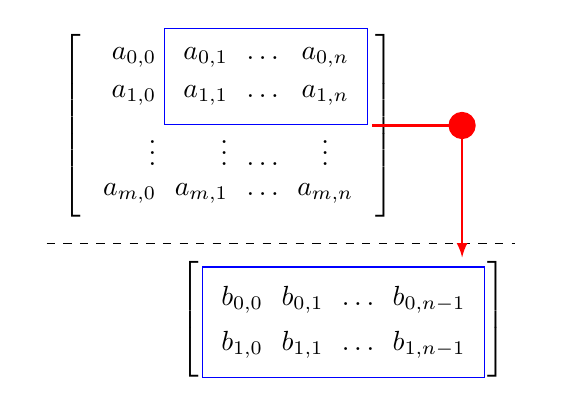
\begin{tikzpicture}[>=latex]
\matrix (M) [matrix of math nodes,left delimiter={[}, right delimiter={]},
matrix anchor=west,  
column 1/.style={anchor=base east},
column 2/.style={anchor=base east},
column 3/.style={anchor=base east}] at (0,0.3)
{
	a_{0,0} & a_{0,1} & \ldots & a_{0,n}\\
	a_{1,0} & a_{1,1} & \ldots & a_{1,n}\\
	\vdots  & \vdots  & \ldots & \vdots \\
	a_{m,0} & a_{m,1} & \ldots & a_{m,n}\\
};
\node  [fit=(M-1-2) (M-2-4), draw, rectangle, blue]{};    
\node (A) at (-0.6,-1.2) {};
\node (B) at (5.6,-1.2) {};
\draw[-,dashed] (A) to (B);
\matrix (N) [matrix of math nodes,left delimiter={[}, right delimiter={]},
matrix anchor=west,  
column 1/.style={anchor=base east},
column 2/.style={anchor=base east},
column 3/.style={anchor=base east}] at (1.5,-2.2)
{
	b_{0,0} & b_{0,1} & \ldots & b_{0,n-1}\\
	b_{1,0} & b_{1,1} & \ldots & b_{1,n-1}\\
};
\node  [fit=(N-1-1) (N-2-4), draw, rectangle, blue]{};  
\node[draw,circle,red,fill=red,minimum size=0.1em] (C) at (4.8,0.3) {};
\node (D) at (4.8,-1.5) {};
\draw [-,red,thick] (M.east) to (C);
\draw [->,red,thick] (C) to (D);
\end{tikzpicture}
\end{column}
\begin{column}{0.5\columnwidth}
\begin{itemize}
	\item The subarray may be situated anywhere within the full array,
	\item The subarray may be of any (nonzero) size up to the size of the larger array (it
	has to be confined within the original array!)
	\item Note that a C program may use Fortran order and a Fortran program may use C order.
\end{itemize}
\end{column}
\end{columns}
\end{onlyenv}
\end{frame}

\begin{frame}[fragile]{Datatype constructors -- Example}
As a first example we extract and communicate a subarray of a 1D array.
\begin{columns}
	\begin{column}{0.50\textwidth}
\footnotesize
\begin{onlyenv}<1->
\begin{minted}{c}
int myrank;
MPI_Status status;
MPI_Datatype subarray;
int array[9] = { -1, 1, 2, 3, -2, 
-3, -4, -5, -6 };
int array_size[] = {9};
int array_subsize[] = {3};
int array_start[] = {1};
\end{minted}
\end{onlyenv}
\begin{onlyenv}<2->
\begin{minted}{c}
MPI_Init(&argc, &argv);
MPI_Type_create_subarray(1, array_size, 
 array_subsize, array_start, 
 MPI_ORDER_C, MPI_INT, &subarray);
MPI_Type_commit(&subarray);
\end{minted}
\end{onlyenv}
\begin{onlyenv}<3->
\begin{minted}{c}
MPI_Comm_rank(MPI_COMM_WORLD, &myrank);
if (myrank == 0){
 MPI_Send(array, 1, subarray, 1, 123, 
  MPI_COMM_WORLD);
}
\end{minted}
\end{onlyenv}
\end{column}
\begin{column}{0.5\textwidth}
\begin{itemize}
\item<1-> We start by producing a subarray for a 1D array \mintinline{c}{int array[9]}
\item<2-> We select the subarray made of 3 elements (\mintinline{c}{int array_subsize[]={3};}), starting from the first position (\mintinline{c}{int array_start[]={1}}) from an array of 9 elements (\mintinline{c}{int array_size[]={9}});
\item<3-> From the process with \mintinline{c}{myrank = 0;} we send the subarray taken from the variable \mintinline{c}{array} to the process with rank 1.
\end{itemize}
\end{column}
\end{columns}
\end{frame}

\begin{frame}[fragile]{Datatype constructors -- Example}
As a first example we extract and communicate a subarray of a 1D array.
\begin{columns}
\begin{column}{0.55\textwidth}
\footnotesize
\begin{onlyenv}<1->
\begin{minted}{c}
else if (myrank == 1){
 for (int i=0; i<9; i++)
  array[i] = 0;
 MPI_Recv(array, 1, subarray, 0, 123, 
  MPI_COMM_WORLD, &status);
 for (int i=0; i<9; i++)
  printf("array[%d] = %d\n", i, array[i]);
 fflush(stdout);
}
\end{minted}
\end{onlyenv}
\begin{onlyenv}<2->
\begin{minted}{c}
MPI_Type_free(&subarray);
MPI_Finalize();
\end{minted}
\end{onlyenv}
\end{column}
\begin{column}{0.45\textwidth}
\begin{itemize}
\item<1-> The process with \mintinline{c}{myrank = 1;} receives the variable and stores it into its version of the variable \mintinline{c}{array}.
\item<2-> In conclusion we deallocate the \mintinline{c}{subarray} type, and finalize the MPI environment.
\end{itemize}
\end{column}
\end{columns}
\begin{itemize}
	\item<3-> When we run the code we print in output the \mintinline{c}{array} with values
	\mint{bash}{array[0] = 0 array[1] = 1 array[2] = 2 array[3] = 3 
	}
	\mint{bash}{array[4] = 0 ...}
	that are the elements in position 2 to 4 of
	\begin{center}
	\verb|array[9] = { -1, 1, 2, 3, -2,-3, -4, -5, -6 };|
	\end{center}
\end{itemize}
\end{frame}

\begin{frame}[fragile]{Datatype constructors -- Example}
\begin{itemize}
	\item We could have been more clever in the receveing phase:
\end{itemize}
\begin{columns}
\begin{column}{0.5\columnwidth}
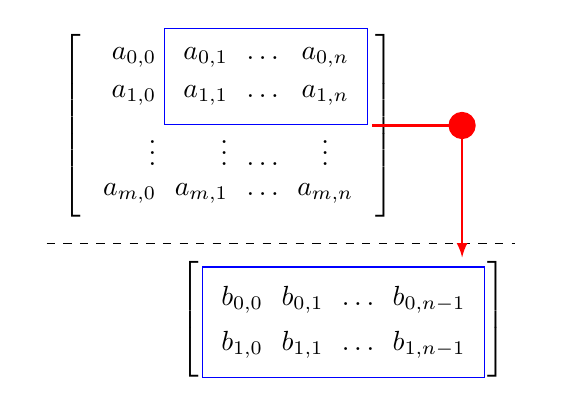
\begin{tikzpicture}[>=latex]
\matrix (M) [matrix of math nodes,left delimiter={[}, right delimiter={]},
matrix anchor=west,  
column 1/.style={anchor=base east},
column 2/.style={anchor=base east},
column 3/.style={anchor=base east}] at (0,0.3)
{
a_{0,0} & a_{0,1} & \ldots & a_{0,n}\\
a_{1,0} & a_{1,1} & \ldots & a_{1,n}\\
\vdots  & \vdots  & \ldots & \vdots \\
a_{m,0} & a_{m,1} & \ldots & a_{m,n}\\
};
\node  [fit=(M-1-2) (M-2-4), draw, rectangle, blue]{};    
\node (A) at (-0.6,-1.2) {};
\node (B) at (5.6,-1.2) {};
\draw[-,dashed] (A) to (B);
\matrix (N) [matrix of math nodes,left delimiter={[}, right delimiter={]},
matrix anchor=west,  
column 1/.style={anchor=base east},
column 2/.style={anchor=base east},
column 3/.style={anchor=base east}] at (1.5,-2.2)
{
b_{0,0} & b_{0,1} & \ldots & b_{0,n-1}\\
b_{1,0} & b_{1,1} & \ldots & b_{1,n-1}\\
};
\node  [fit=(N-1-1) (N-2-4), draw, rectangle, blue]{};  
\node[draw,circle,red,fill=red,minimum size=0.1em] (C) at (4.8,0.3) {};
\node (D) at (4.8,-1.5) {};
\draw [-,red,thick] (M.east) to (C);
\draw [->,red,thick] (C) to (D);
\end{tikzpicture}
\end{column}
\begin{column}{0.5\columnwidth}
\begin{itemize}
\item If we look back at the figure the receveing array was instead an array object of the received size,
\item Nevertheless, if we expect to use the the new datatype \mintinline{c}{subarray} on the receiving end we have to use an array with global size
equal to the one used to build the type
\end{itemize}
\end{column}
\end{columns}
\begin{itemize}
	\item We can do it in a slightly different way to match what is depicted in the figure:
\end{itemize}
\begin{minted}{c}
 int receivearray[3];
 MPI_Recv(receivearray, 3, MPI_INT, 0, 123, 
  MPI_COMM_WORLD, &status);	
\end{minted}
\end{frame}

\begin{frame}[fragile]{Datatype constructors -- Exercise}
Let us use the \mintinline{c}{MPI_Type_create_subarray} routine to extract a 2D subarray from a 2D array.
\begin{enumerate}
	\item We want to be a little more general than we have been for the 1D array case, thus let us define first two functions:
	\begin{itemize}
		\item a function \mintinline{c}{int **allocarray(int n)} that allocates a $n\times n$ array;
		\item a function \mintinline{c}{void printarr(int **array, int n, char *str)} that takes as input the address of a 2D array \mintinline{c}{int **array}, its size \mintinline{c}{int n}, and a string with the name of the array for printing everything to screen.
	\end{itemize}
	\item Then processor 0 initializes (and populates) the \mintinline{c}{bigarray}, build the new data type with the \mintinline{c}{MPI_Type_create_subarray} routine, prints it in output and sends the data to a (smaller) array on processor 1.
	\item On the other side, processor 1 initializes the memory for the \mintinline{c}{subarray}, receives the message from process 0, prints it in output and terminates.
\end{enumerate}
\begin{itemize}
	\item You have an ``skeleton code'' in the \mintinline{bash}{subarray2Darray.c} file in the code folder.
\end{itemize}
\end{frame}

\begin{frame}[fragile]{Datatype constructors -- Exercise}
\small
The function to dynamically allocate a 2D array can be written as:
\begin{minted}{c}
int **allocarray(int n) {
int *rows = malloc(n*n*sizeof(int));
int **arr2D = malloc(n*sizeof(int *));
for (int i=0; i<n; i++)
  arr2D[i] = &(rows[i*n]);
return arr2D;
}
\end{minted}
while the function to print a given $n\times n$ array can be obtained as
\begin{minted}{c}
void printarr(int **array, int n, char *str) {
 printf("-- %s --\n", str);
 for (int i=0; i<n; i++) {
  for (int j=0; j<n; j++) {
   printf("%3d ", array[i][j]);
  }
  printf("\n");
 }
}
\end{minted}
\end{frame}

\begin{frame}[fragile]{Datatype constructors -- Exercise}
\small\vspace{-1em}
On the processor with \mintinline{c}{rank = 0;} we initialize (and populate) the \mintinline{c}{bigarray}, build the new data type with the \mintinline{c}{MPI_Type_create_subarray} routine, then we print it in output and sends the data to a (smaller) array on processor 1.
\begin{minted}{c}
int **bigarray = allocarray(bigsize);
for (int i=0; i<bigsize; i++)
 for (int j=0; j<bigsize; j++)
  bigarray[i][j] = i*bigsize+j;
printarr(bigarray, bigsize, " Sender: Big array ");
\end{minted}
and then the main part:
\begin{onlyenv}<1>
\begin{minted}{c}
MPI_Datatype mysubarray;
// We choose the coordinate from which we start the communication:
int starts[ ] = {};
int subsizes[ ]  = {}; // The size of the square subarray to 
                       // communicate
int bigsizes[ ]  = {}; // The size of the big square array
MPI_Type_create_subarray(); // We create the subarray type
MPI_Type_commit(); // We commit it
MPI_Send(); // We send the subarray to process 1
MPI_Type_free(); // We deallocate the type
\end{minted}
\end{onlyenv}
\begin{onlyenv}<2>
\begin{minted}{c}
MPI_Datatype mysubarray;
int starts[2] = {5,3};
int subsizes[2]  = {subsize,subsize};
int bigsizes[2]  = {bigsize,bigsize};
MPI_Type_create_subarray(2, bigsizes, subsizes, starts,
MPI_ORDER_C, MPI_INT, &mysubarray);
MPI_Type_commit(&mysubarray);
MPI_Send(&(bigarray[0][0]),1,mysubarray,1,tag,MPI_COMM_WORLD);
MPI_Type_free(&mysubarray);
\end{minted}
\end{onlyenv}
\end{frame}

\begin{frame}[fragile]{Datatype constructors -- Exercise}
\small\vspace{-1em}
Processor 1 initializes the memory for the \mintinline{c}{subarray}, receives the message from process 0, prints it in output and terminates.
\begin{onlyenv}<1>
\begin{minted}{c}
// Now we are rank 1: we first allocate the array for 
// receiving the message from rank 0 (it has to be a 
// square array of size subsize^2):
int **subarray = allocarray();
// with a double for loop we put to zero the entries of the 
// receiveing array:
for (int i=0; i<subsize; i++)
 for (int j=0; j<subsize; j++)
  subarray[i][j] = 0;
// We receive the data in the subarray we have allocated
MPI_Recv();
// We print what we have received:
printarr(subarray, subsize,"Receiver: Subarray -- after receive");
\end{minted}
\end{onlyenv}
\begin{onlyenv}<2>
\begin{minted}{c}
// Now we are rank 1: we first allocate the array for 
// receiving the message from rank 0 (it has to be a 
// square array of size subsize^2):
int **subarray = allocarray(subsize);
// with a double for loop we put to zero the entries of the 
// receiveing array:
for (int i=0; i<subsize; i++)
 for (int j=0; j<subsize; j++)
  subarray[i][j] = 0;
// We receive the data in the subarray we have allocated
MPI_Recv(&(subarray[0][0]), subsize*subsize, MPI_INT, 0, 
  tag, MPI_COMM_WORLD, &status);
// We print what we have received:
printarr(subarray, subsize,"Receiver: Subarray -- after receive");
\end{minted}
\end{onlyenv}	
\end{frame}

\begin{frame}[fragile]{Datatype constructors -- (Further) Exercise(s)}
Observe that:
\begin{itemize}
	\item we have freed the \mintinline{c}{mysubarray} (\mintinline{c}{MPI_Type_free(&mysubarray);}) right after sending a data with this type, this operation is \emph{safe} since it does not interfere with instantiated communications.
	\item to free the dynamically allocated arrays we do it in the order:
\begin{minted}{c}
free(bigarray[0]);
free(bigarray);
\end{minted}
	i.e., we first free the memory allocated for the rows, then we free the pointer to the whole array. We need to free the memory from inside/out, otherwise we loose the inner pointers!
\end{itemize}

\onslide<2>{
Some extensions of the previous exercise could be:
\begin{itemize}
\item Generalize the construction of the array to a rectangular array of size $n \times m$,
\item Try allocating and sending array with more than 2D dimensions,
\end{itemize}
}
\end{frame}

\section{Numerical integration of the H\'enon--Heiles model}

\begin{frame}{Numerical integration of the H\'enon--Heiles model}
As a concluding example we consider the problem of integrating an (a system of) ODE(s) for different values of the parameters defining it.
\begin{block}<2->{Parallel integration of ODEs}
There exists algorithms (and libraries) that permits to actually integrate in parallel an ODE, they exploit
\begin{itemize}
	\item parallelism across the method, e.g., substantially rewrite the sequential nature of integration procedure: exploit independent stages of multi--stage algorithms, 
	\item parallelism across the system, e.g., different evolution time for the ODEs: waveform relaxation.
	\item parallelism across the steps, e.g., we have a huge time domain that we want to divide into parallel processes: parallel in time algorithm.
\end{itemize}
\end{block}

\onslide<3>{We are going to treat a much simpler usage of parallelism: having to integrate the same ODE(s) for different values of some parameters.}
\end{frame}

\begin{frame}{Numerical integration of the H\'enon--Heiles model}
Let us remain on the concrete, the ODEs we want to integrate is obtained from the Hamiltonian
\begin{equation*}
	H(\mathbf{p},\mathbf{q}) = \frac{\omega_1}{2}(q_1^2+p_1^2) + \frac{\omega_2}{2} (q_2^2 + p_2^2) + p_1^2 q_2 - \frac{1}{3}p_2^3, \quad \omega_1,\omega_2 \in \mathbb{R},
\end{equation*}
where the $q_i$ denotes the position coordinates, the $p_i$ the momentum coordinates, and from which we obtain the Hamilton's equations
\begin{equation*}
\begin{cases}
	\dot{q}_1 = \frac{\partial H}{\partial p_1} = 2 p_1 q_2 + \omega_1 p_1,\\
	\dot{q}_2 = \frac{\partial H}{\partial p_2} = \omega _2 p_2 -\frac{2 p_2}{3},\\
	\dot{p}_1 = -\frac{\partial H}{\partial q_1} = - \omega _1 q_1 ,\\
	\dot{p}_2 = -\frac{\partial H}{\partial q_2} = -p_1^2- \omega _2 q_2.
\end{cases}
\end{equation*}
and we are interested in integrating it for different values of the constants $\omega_1,\omega_2$, and different values of the energy $E$.
\vfill
\onslide<2>{What are the operation that our (parallel) software should perform?}
\end{frame}

\begin{frame}{Numerical integration of the H\'enon--Heiles model}
The ``general idea'' for performing such task can be summarized as:
\begin{enumerate}
	\item Processor 0 reads the list of parameters in input for each instance of the problem,
	\item Processor 0 \emph{scatters} such data to every other process in the pool,
	\item Each processor from \mintinline{c}{0,...,size-1} executes its own integration,
	\item Processor 0 \emph{gathers} the results from all the processors,
	\item Processor 0 writes the result on a file in a format that can be used to plot the \mintinline{c}{size} different solutions.  
\end{enumerate}
\onslide<2->{Now, we need to precise this statements\ldots and the devil is in the details}
\begin{itemize}
	\item<3-> To decide what parameters we need, we first need to decide what method we want to use for the integration,
	\item<4-> What type of method do we need? \onslide<5>{ We need conservation of energy, so we need a \alert{\emph{symplectic} method}.}
\end{itemize}
\end{frame}

\begin{frame}{Numerical integration of the H\'enon--Heiles model}

\begin{block}{Symplectic integrators}
A symplectic integrator is a numerical integration scheme for Hamiltonian systems, i.e., it is used to integrate equations of the form:
\begin{equation*}
	\dot{q}_i = \frac{\partial H}{\partial p_i}, \quad \dot{p}_i = -\frac{\partial H}{\partial q_i}, \quad i=1,\ldots,n.
\end{equation*}
This is a method for which, under opportune constraints on its parameters, a solution on a symplectic manifold is computed. 
\end{block}

\begin{itemize}
	\item<2-> a symplectic integrator conserves the value of $H$ along the computed trajectories,
	\item<3-> it conserves the two--from $d\mathbf{p} \wedge d\mathbf{q}$.
	\item<4-> we are doing it \emph{numerically} thus ``conserves'' means up to the accuracy of method, i.e., it conserves a \emph{numerical} Hamiltonian (\ldots usually a perturbation of the original one)
\end{itemize}

\end{frame}

\begin{frame}{Numerical integration of the H\'enon--Heiles model}
For our test program we will use the \alert{leapfrog method}\footnote{\scriptsize See, e.g., J. Laskar\ and\ P. Robutel, High order symplectic integrators for perturbed Hamiltonian systems, Celestial Mech. Dynam. Astronom. {\bf 80} (2001), no.~1, 39--62.}. We divide the integration interval $[0,T_{\text{max}}]$ in $n$ intervals, i.e., $dt = T_{\text{max}}/n$, and consider the evaluation of $\{p_i^{(n)},q_i^{(n)}\}_{i=1}^{2}$, for $n=0,\ldots,n$, on the points $t_i = i dt$.

The method is then obtained as:
\begin{equation*}
	\begin{cases}
	p^{(n+1/2)}_1 = p^{(n-1)}_1 + \frac{\omega_1}{2} q_1^{(n-1)} dt,\\
	p^{(n+1/2)}_2 = p^{(n-1)}_2 + \frac{\omega_2}{2} q_2^{(n-1)} dt,\\
	q^{(n)}_1 = q^{(n-1)}_1 - (\omega_1 p_1^{(n+1/2)} + 2 p_1^{(n+1/2)} p_2^{(n+1/2)} ) dt,\\
	q^{(n)}_2 = q^{(n-1)}_2 - (\omega_2 p_2^{(n+1/2)} + [p_1^{(n+1/2)}]^2 + [p_2^{(n+1/2)}]^2 ) dt,\\
	p^{(n)}_1 = p^{(n+1/2)}_1 + \frac{\omega_1}{2} q_1^{(n)} dt,\\
	p^{(n)}_2 = p^{(n+1/2)}_2 + \frac{\omega_2}{2} q_2^{(n)} dt,\\	  
	\end{cases}
\end{equation*}
This is a symplectic method of order 1!
\end{frame}

\begin{frame}[fragile]{Numerical integration of the H\'enon--Heiles model}
\small\vspace{-1.5em}
\begin{itemize}
	\item Observe that the first and the last block are the same computation on different inputs, therefore we can perform it as:
\end{itemize}\vspace{-1em}
\begin{minted}{c}
void kin_flow(double p[2], double q[2], 
 double omega[2], double dt){
  p[0] += omega[0] * q[0] * 0.5 * dt;
  p[1] += omega[1] * q[1] * 0.5 * dt;}
\end{minted}
\begin{itemize}
	\item then the central block for updating the $q_i$ can be coded as
\end{itemize}\vspace{-1em}
\begin{minted}{c}
void pot_flow(double p[2], double q[2], double omega[2], 
  double dt){
 q[0] -= ( omega[0] * p[0] + 2 * p[0] * p[1] ) * dt;
 q[1] -= ( omega[1] * p[1] + pow(p[0],2) - pow(p[1],2) ) * dt;}
\end{minted}
\begin{itemize}
	\item A complete step of the integration is then given by
\end{itemize}\vspace{-1em}
\begin{minted}{c}
void leapfrog(double p[2], double q[2], double omega[2], 
 double dt){
kin_flow(p, q, omega, dt);
pot_flow(p, q, omega, dt);
kin_flow(p, q, omega, dt);}
\end{minted}
\end{frame}

\begin{frame}[fragile]{Numerical integration of the H\'enon--Heiles model}
\small\vspace{-1em}
Then to integrate our Hamiltonian system we repeat the routine performing one step $n$ times (\mintinline{c}{int numberofsteps} times)
\begin{minted}{c}
for(int i=1; i<=numberofsteps; i++) {
 leapfrog(p, q, omega, dt);
 energy_at_time_t = compute_energy(p, q, omega);
 delta_energy[i] = energy_at_time_t - initialenergy;
}
\end{minted}
\vspace{-1em}
\begin{itemize}
\item we have coded the algorithm in a way that does not store the values of $\{p_i^{(j)},q_i^{(j)}\}_{i=1,2}^{j=1,\ldots,n}$, therefore we need to compute the energy at each integration step,
\item the \emph{energy} is nothing more than the value of the Hamiltonian on the current values of $p_i$ and $q_j$, i.e.,
\end{itemize}
\begin{minted}{c}
double compute_energy(double p[2], double q[2], double omega[2]){
int i; double ris = 0;
for(i=0; i<2; i++)
 ris += omega[i] * ( pow(p[i],2) + pow(q[i],2) ) / 2;
ris += p[1] * ( pow(p[0],2) - pow(p[1],2) / 3 );
return ris;
}
\end{minted}
\end{frame}

\begin{frame}[fragile]{Numerical integration of the H\'enon--Heiles model}
The last part of the sequential algorithm we need to precise regards the initial conditions and the initial energy:
\begin{minted}{c}
delta_energy[0] = initialenergy - omega[1]*(pow(p0[1],2)
 + pow(q0[1],2))/2.0 + pow(p0[1],3)/3.0;
q0[0] = sqrt(2.0*delta_energy[0]/omega[0]);
p0[0] = 0;
for(int i=0; i<2; i++) {
 p[i] = p0[i];
 q[i] = q0[i];
}
\end{minted}
in which we are assuming to know:
\begin{itemize}
\item the values of \mintinline{c}{p0[1]}, and \mintinline{c}{q0[1]},
\item the initial value of the energy \mintinline{c}{initialenergy},
\item to complete the information we need as input also the values \mintinline{c}{omega[0]}, \mintinline{c}{omega[1]}, the maximum time of integration \mintinline{c}{tmax}, and either the value of \mintinline{c}{dt} or the number of intervals \mintinline{c}{n}.
\end{itemize}
\end{frame}

\begin{frame}[fragile]{Numerical integration of the H\'enon--Heiles model}
Let us look again at our list:
\begin{enumerate}
	\item Processor 0 reads the list of parameters in input for each instance of the problem,
	\item Processor 0 \emph{scatters} such data to every other process in the pool,
	\item Each processor from \mintinline{c}{0,...,size-1} executes its own integration,
	\item Processor 0 \emph{gathers} the results from all the processors,
	\item Processor 0 writes the result on a file in a format that can be used to plot the \mintinline{c}{size} different solutions.  
\end{enumerate}
we have solved how to perform the integration at step 3, and we know what parameters in input we need, namely:
\begin{itemize}
	\item \mintinline{c}{omega[0]}, \mintinline{c}{omega[1]}, \mintinline{c}{initialenergy}, \mintinline{c}{p0[1]}, \mintinline{c}{q0[1]}, \mintinline{c}{tmax}, \mintinline{c}{dt}
	\item we want to read the the input for all the processors on \mintinline{c}{rank 0}, therefore we decide to produce our input file in the following form:
	\begin{itemize}
		\item the first line will tell us how many sets of parameters we have,
		\item the following lines, in groups by seven, will give us all the various parameters in the order above, one for each line.
	\end{itemize}
\end{itemize}
\end{frame}

\begin{frame}[fragile]{Numerical integration of the H\'enon--Heiles model}
\small
\begin{columns}
\begin{column}{0.25\textwidth}
\scriptsize
Input file: \mintinline{bash}{henonheiles.inp}
\begin{verbatim}
3
1 
0.6180339887498948482
0.03
0.35
0.
1.
0.1
1
0.6180339887498948482
0.03
0.35
0.
1.
0.1
1 
0.6180339887498948482
0.03
0.35
0.
1.
0.01
\end{verbatim}
\end{column}
\begin{column}{0.75\textwidth}
\begin{minted}{c}
if(myrank == 0){
 FILE *ifp; char line[300];
 int numberoftests, i=0;
 ifp = fopen("henonheiles.inp","r");
 if (ifp == NULL) {
  fprintf(stderr, 
   "Can't open input file henonheiles.inp!\n");
  MPI_Finalize(); return 1;
 }
 fgets(line, 300, ifp); 
 sscanf(line,"%d",&numberoftests);
 readdata = (double *) 
   malloc( sizeof(double)*7*numberoftests );
 while(fgets(line, 300, ifp)!=NULL) {
 readdata[i]=atof(line);
 i++;
 }
 fclose(ifp);
}
\end{minted}
\end{column}
\end{columns}
\end{frame}

\begin{frame}[fragile]{Numerical integration of the H\'enon--Heiles model}\small
At this point the array \mintinline{c}{readdata} contains all the input value, we need now to send to each processor in \mintinline{c}{MPI_COMM_RANK} for \mintinline{c}{0,...,size-1} the relative seven values:
\begin{minted}{c}
double input[7];
MPI_Scatter(readdata,7,MPI_DOUBLE,input,7,MPI_DOUBLE,0,
  MPI_COMM_WORLD);
\end{minted}
\begin{itemize}
	\item this function has to be called by each processor,
	\item after the completion of the communication processor $j$ has the $j$th group of 7 inputs (\mintinline{c}{omega[0]}, \mintinline{c}{omega[1]}, \mintinline{c}{initialenergy}, \mintinline{c}{p0[1]}, \mintinline{c}{q0[1]}, \mintinline{c}{tmax}, \mintinline{c}{dt}),
\end{itemize}
\begin{onlyenv}<2>
\vspace{-0.3em}On each processor we can populate the (local) inputs with the values:
\begin{minted}{c}
double omega[2],initialenergy,p0[2],q0[2],tmax,dt;
omega[0] = input[0]; omega[1] = input[1];
initialenergy = input[2]; p0[1] = input[3]; q0[1] = input[4];
tmax = input[5]; dt = input[6];
\end{minted}
\vspace{-0.3em}and compute the number of steps by doing: \mint{c}{int numberofsteps = tmax/dt;}
\end{onlyenv}
\end{frame}

\begin{frame}[fragile]{Numerical integration of the H\'enon--Heiles model}
We need now to gather the array \mintinline{c}{delta_energy} containing the error on the energy from each processor.
\begin{itemize}
	\item \alert{Note:} the size of \mintinline{c}{delta_energy} may be different on each processor!
	\item<2-> we can use the \mintinline{c}{MPI_Gatherv} function to accommodate this issue, \alert{but} this requires knowing the length of each array!
	\item<3-> we can first share this information between all the processors by using an \mintinline{c}{MPI_Allgather} that will store this information on the array \mint{c}{int *intervals_for_process;} by calling:
\begin{minted}{c}
intervals_for_process=(int *) malloc(sizeof(int)*size);
MPI_Allgather(&numberofsteps,1,MPI_INT,
  intervals_for_process,1,MPI_INT,MPI_COMM_WORLD);
\end{minted}
after this call every processor will have the information regarding the number of nodes computed by each processor.
\end{itemize}

\end{frame}

\begin{frame}[fragile]{Numerical integration of the H\'enon--Heiles model}
\small
We put together the ingredients needed for the \mintinline{c}{MPI_Gatherv}
\begin{columns}
\begin{column}{0.5\columnwidth}
\begin{minted}{c}
if (myrank == 0){
 stride = (int *) 
   malloc(sizeof(int)*size);
 for(int i = 0; i < size; i++){
  grandtotal += 
    intervals_for_process[i];
 if(i==0){
  stride[i] = 0;
 }else{
  stride[i] = stride[i-1]
   +intervals_for_process[i-1];
 }
}
every_delta_energy = (double *) 
 malloc(sizeof(double)*
  (grandtotal+size));
}
\end{minted}
\end{column}
\begin{column}{0.5\columnwidth}
\begin{itemize}
	\item Observe that we have allocated the memory for the receive only on the
	root processor, it would have been a waste of resources allocating it everywhere!
	\item We will need to put the received vectors with the correct spacing in the receiving buffer  
	(\mintinline{c}{every_delta_energy}), thus we need to define the opportune stride  
	(\mintinline{c}{recevbuf +} \mintinline{c}{stride[i]*extent[recevtype]})
	\item all this information are needed only on the \mintinline{c}{root} process, so it is safe to
	define their value only on this rank.
\end{itemize}
\end{column}
\end{columns}
\end{frame}

\begin{frame}[fragile]{Numerical integration of the H\'enon--Heiles model}
We have all the pieces needed for the \mintinline{c}{MPI_Gatherv}:
\begin{minted}{c}
MPI_Gatherv(delta_energy,numberofsteps,MPI_DOUBLE,
 every_delta_energy, intervals_for_process,stride,
 MPI_DOUBLE,0,MPI_COMM_WORLD);
\end{minted}
\begin{itemize}
	\item each process will contribute with its own local \mintinline{c}{delta_energy} (that is an array of \mintinline{c}{numberofsteps} \mintinline{c}{double}s),
	\item everything will end up in the \mintinline{c}{every_delta_energy}, it is going to receive from $j$th processor \mintinline{c}{intervals_for_process[j]} \mintinline{c}{double}s,
	\item the received values will be placed contiguously as dictated by the \mintinline{c}{stride} array.
\end{itemize}
\onslide<2>{To conclude our code, we need only to print every result in its own file.}
\end{frame}

\begin{frame}[fragile]{Numerical integration of the H\'enon--Heiles model}
\small
The writing is completely mechanical at this point:
\begin{minted}{c}
if (myrank == 0){
 FILE *ofp;
 int glob_counter = 0;
 char filename[200];
 for(int i = 0; i < size;i++){
  sprintf(filename,"energy_process_%d.dat",i);
  ofp = fopen(filename,"w+");
  for(int j=0; j < intervals_for_process[i]; j++){
   fprintf(ofp, "     %le      %le\n",
   j * readdata[i*7+6],
   every_delta_energy[glob_counter]);
   glob_counter++;
  }
  fclose(ofp);
 }
 free(readdata); free(every_delta_energy);
}
free(intervals_for_process);
\end{minted}
\end{frame}

\begin{frame}{Numerical integration of the H\'enon--Heiles model}
\begin{columns}
	\begin{column}{0.45\columnwidth}
		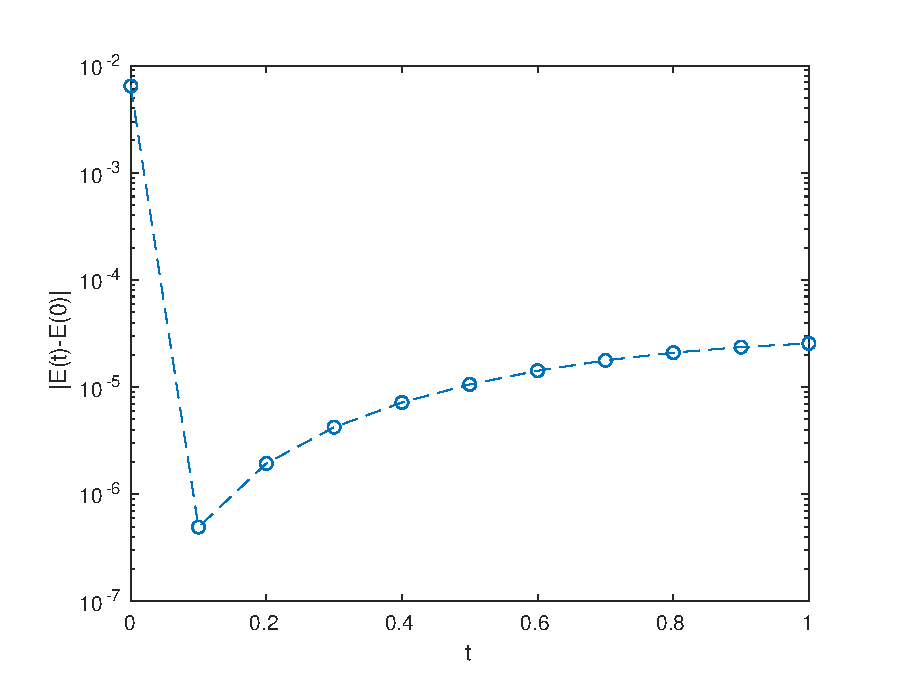
\includegraphics[width=\columnwidth]{figure1.eps}
		
		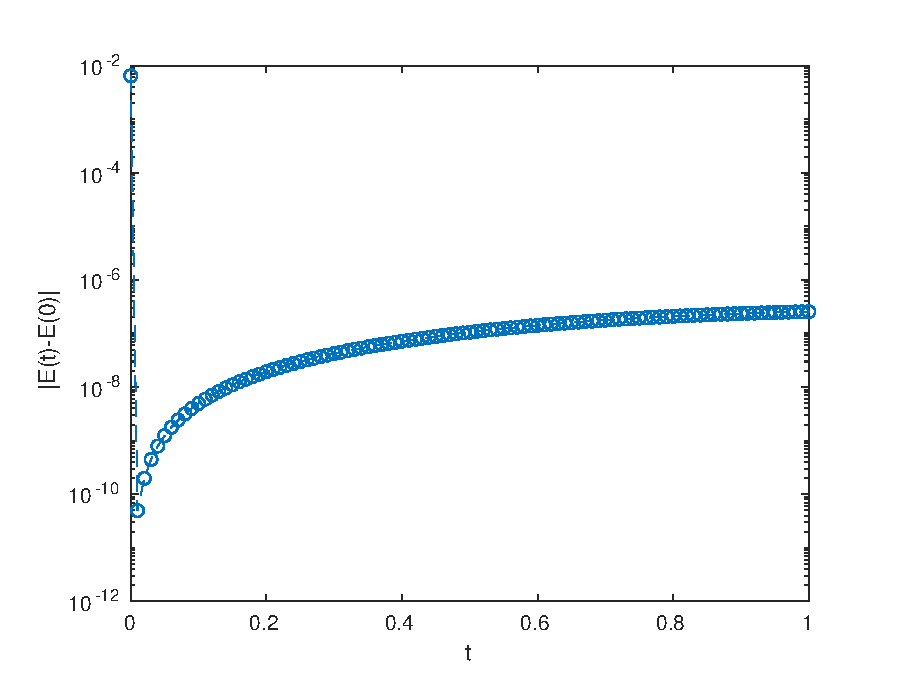
\includegraphics[width=\columnwidth]{figure2.eps}
	\end{column}
\begin{column}{0.55\columnwidth}
As usual, this code is not perfect, and there are several possible improvement
\begin{itemize}
	\item Written in this way we need to pay attention to the ratio between the number of processors and parameter sets,
	\item We could use a reduce operation (\mintinline{c}{MPI_Reduce}) to get (instead of all the array of the errors) a norm or some other meaningful statistics,
	\item We may modify it to get instead the value of the positions $p_i$, or the moments $q_i$,
	\item \ldots
\end{itemize}
\end{column}
\end{columns}
\end{frame}

\section{``They're moving in herds. They do move in herds.''}

\begin{frame}{``They're moving in herds. They do move in herds.''}
\small
\only<1>{\centering 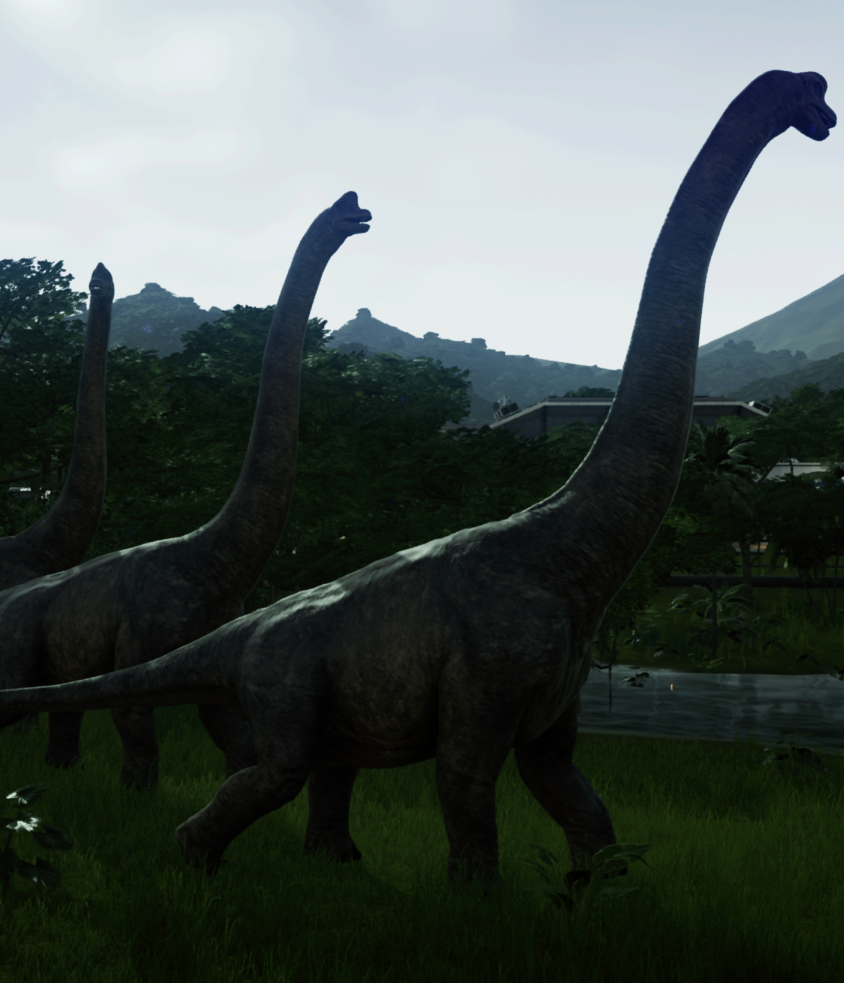
\includegraphics[width=0.6\columnwidth]{dinosauri.png}}
\only<2->{
There exists many libraries with parallel capabilities for scientific computing.
\begin{itemize}
\item[LA] Parallel Basic Linear Algebra Subprograms
	\begin{itemize}
		\item \texttt{ScaLAPACK}: \href{http://www.netlib.org/scalapack}{www.netlib.org/scalapack}
		\item \alert<3>{\texttt{PSBLAS}}: \href{https://github.com/sfilippone/psblas3}{github.com/sfilippone/psblas3}
		\item \texttt{PETSc}: \href{https://www.mcs.anl.gov/petsc}{www.mcs.anl.gov/petsc}
	\end{itemize}
\item[Solvers] Solvers for Linear and Nonlinear equations
	\begin{itemize}
		\item \texttt{Hypre}: \href{https://computing.llnl.gov/projects/hypre-scalable-linear-solvers-multigrid-methods}{computing.llnl.gov/projects/hypre-scalable-linear-solvers-multigrid-methods}
		\item \alert<3>{\texttt{AMG4PSBLAS}}: \href{https://github.com/sfilippone/amg4psblas}{github.com/sfilippone/amg4psblas}
		\item \texttt{MUMPS}: \href{http://mumps.enseeiht.fr/}{mumps.enseeiht.fr/}
		\item \texttt{Trilinos}: \href{https://trilinos.github.io/}{trilinos.github.io/}
		\item \texttt{SUNDIALS}: \href{https://computing.llnl.gov/projects/sundials}{computing.llnl.gov/projects/sundials}
	\end{itemize}
\item[Repos]
\begin{itemize}
	\item \href{https://software.llnl.gov}{software.llnl.gov}
	\item \href{https://developer.nvidia.com/gpu-accelerated-libraries}{developer.nvidia.com/gpu-accelerated-libraries}
	\item \href{https://en.wikipedia.org/wiki/List_of_numerical_libraries}{en.wikipedia.org/wiki/List\_of\_numerical\_libraries}
\end{itemize}
\end{itemize}
}
\end{frame}

\begin{frame}{``They're moving in herds. They do move in herds.''}{Shameless advertisement}

\begin{columns}
\begin{column}{0.3\textwidth}
\centering

\includegraphics[width=0.8\columnwidth]{psctoolkit.png}
\end{column}
\begin{column}{0.7\textwidth}
I am a collaborator on the \texttt{PSCToolkit} project\ldots so give it a try! 

\vfill
If you have either to solve large linear systems in parallel,
or have programs based on BLAS, then these tools can be useful.
\end{column}
\end{columns}

\begin{itemize}
	\item For an introduction on  how to use the libraries there are several recorded webinars: \href{https://psctoolkit.github.io/talks/}{psctoolkit.github.io/talks/}
	\item The website \href{https://psctoolkit.github.io/}{psctoolkit.github.io} contains up-to-date information on software release, webinars, and new developments.
\end{itemize}

\end{frame}

\section{Conclusions}

\begin{frame}{Conclusions}
	What do we do now?
	\begin{itemize}
		\item Find a problem you want to solve \emph{computationally} and in \emph{parallel},
		\item Look for an MPI-enabled library implementing the basic routine you may need,
		\item Enter the never-ending cycle of \alert{scientific software development}:
	\end{itemize}
	\begin{center}
		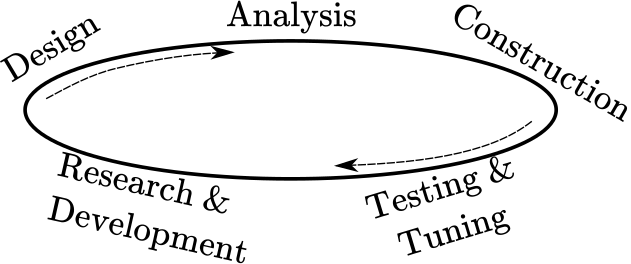
\includegraphics[width=0.5\columnwidth]{softwarecycle.png}
	\end{center}
	Things to read:
	\begin{itemize}
		\item \small Rouson, D., Xia, J., \& Xu, X. (2011). Scientific software design: the object-oriented way. Cambridge University Press.
		\item \small Leiserson, Charles E., et al. There’s plenty of room at the Top: What will drive computer performance after Moore’s law?. Science, 2020, 368.6495.
	\end{itemize}
\end{frame}

\end{document}